\documentclass{beamer}

\mode<presentation> {
	\usetheme{Rochester}
	\setbeamertemplate{footline}[page number]
}

\usepackage{graphicx}
\usepackage{booktabs}

\title[Mind Map PIM]{Mind Map PIM}

\author{A-Cube-N}
\institute[UP]{
	Department of Computer Science, University of Pretoria
}
\date{\today}
\graphicspath{{pictures/}}

\begin{document}
	\section{Interface}
		\begin{frame}
		\frametitle{Interface}
			\begin{figure}
				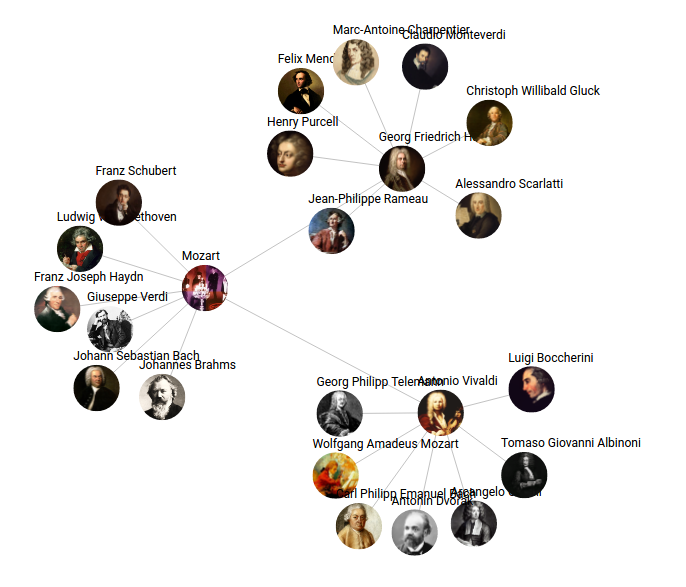
\includegraphics[scale=0.3]{musicroamer.png}
				\caption{Music Roamer layout of a music mind map}
			\end{figure}
		\end{frame}
		
		\begin{frame}
		\frametitle{Initial Design 1}
			\begin{figure}
				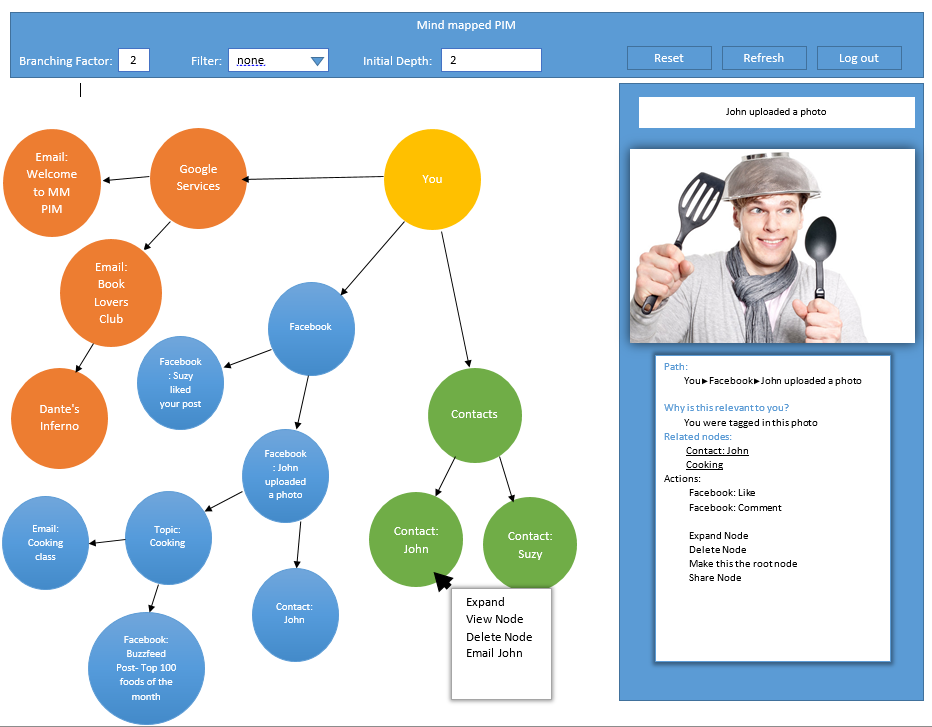
\includegraphics[scale=0.35]{initdesign.png}
			\end{figure}
		\end{frame}
		
		\begin{frame}
		\frametitle{Initial Design 2}
			\begin{figure}
				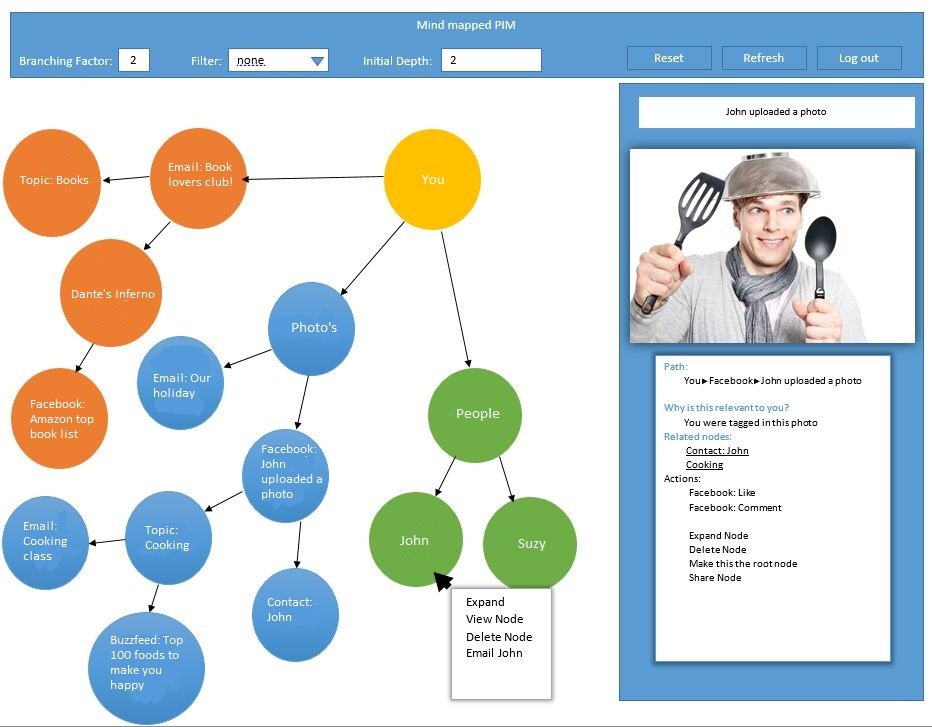
\includegraphics[scale=0.35]{initDesign2.jpg}
			\end{figure}
		\end{frame}

\end{document} 
